\chapter{Joshua 22}

\begin{figure}
  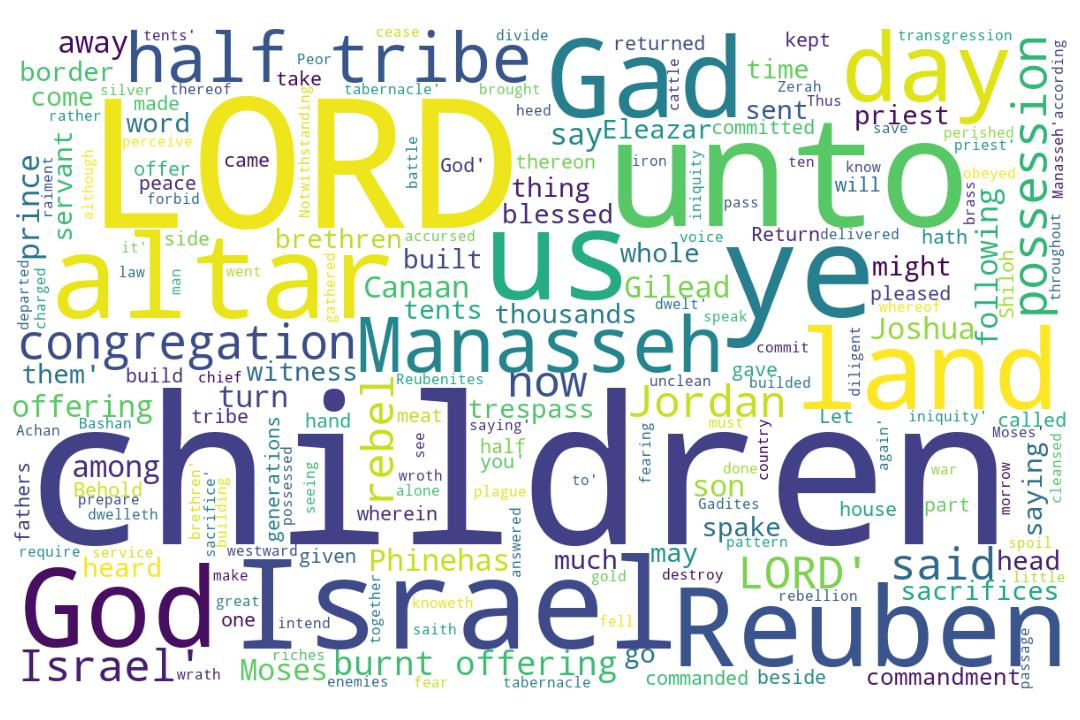
\includegraphics[width=\linewidth]{06OT-Joshua/Joshua22-WordCloud.jpg}
  \caption{Joshua 22 Word Cloud}
  \label{fig:Joshua 22 Word Cloud}
\end{figure}

\marginpar{\scriptsize \centering \fcolorbox{bone}{lime}{\textbf{BACK TO THE OTHER SIDE}}\\ (Joshua 22)

\begin{compactenum}[I.][8]

    \item The \textbf{Two-and-a-Half} \index[scripture]{Joshua!Jsh 22:01}(Jsh 22:1)
    \item \textbf{Toward the East} \index[scripture]{Joshua!Jsh 22:05}(Jsh 22:5)
    \item \textbf{Trouble at Church} \index[scripture]{Joshua!Jsh 22:11}(Jsh 22:11)
    \item \textbf{Tension} \index[scripture]{Joshua!Jsh 22:12}(Jsh 22:12)
    \item A \textbf{Testimony to Unity} \index[scripture]{Joshua!Jsh 22:27}(Jsh 22:27)

\end{compactenum}}

\footnote{\textcolor[rgb]{0.00,0.25,0.00}{\hyperlink{TOC}{Return to end of Table of Contents.}}}\footnote{\href{https://audiobible.com/bible/joshua_22.html}{\textcolor[cmyk]{0.99998,1,0,0}{Joshua 22 Audio}}}\textcolor[cmyk]{0.99998,1,0,0}{Then Joshua called the Reubenites, and the Gadites, and the half tribe of Manasseh,}
[2] \textcolor[cmyk]{0.99998,1,0,0}{And said unto them, Ye have kept all that Moses the servant \fcolorbox{bone}{bone}{of the LORD} commanded you, and have obeyed my voice in all that I commanded you:}
[3] \textcolor[cmyk]{0.99998,1,0,0}{Ye have not left your brethren these many days unto this day, but have kept the charge of the commandment \fcolorbox{bone}{bone}{of the LORD} your God.}
[4] \textcolor[cmyk]{0.99998,1,0,0}{And now the LORD your God hath given rest unto your brethren, as he promised them: therefore now return ye, and get you unto your tents, \emph{and} unto the land of your possession, which Moses the servant \fcolorbox{bone}{bone}{of the LORD} gave you on the other side Jordan.}
[5] \textcolor[cmyk]{0.99998,1,0,0}{But take diligent heed to do the commandment and the law, which Moses the servant \fcolorbox{bone}{bone}{of the LORD} charged you, to love the LORD your God, and to walk in all his ways, and to keep his commandments, and to cleave unto him, and to serve him with all your heart and with all your soul.}
[6] \textcolor[cmyk]{0.99998,1,0,0}{So Joshua blessed them, and sent them away: and they went unto their tents.}\\
\\
\P \textcolor[cmyk]{0.99998,1,0,0}{Now to the \emph{one} half of the tribe of Manasseh Moses had given \emph{possession} in Bashan: but unto the \emph{other} half thereof gave Joshua among their brethren on this side Jordan westward. And when Joshua sent them away also unto their tents, then he blessed them,}
[8] \textcolor[cmyk]{0.99998,1,0,0}{And he spake unto them, saying, Return with much riches unto your tents, and with very much cattle, with silver, and with gold, and with brass, and with iron, and with very much raiment: divide the spoil of your enemies with your brethren.}\\
\\
\P \textcolor[cmyk]{0.99998,1,0,0}{And the children of Reuben and the children of Gad and the half tribe of Manasseh returned, and departed from the children of Israel out of Shiloh, which \emph{is} in the land of Canaan, to go unto the country of Gilead, to the land of their possession, whereof they were possessed, according to the word \fcolorbox{bone}{bone}{of the LORD} by the hand of Moses.}\\
\\
\P \textcolor[cmyk]{0.99998,1,0,0}{And when they came unto the borders of Jordan, that \emph{are} in the land of Canaan, the children of Reuben and the children of Gad and the half tribe of Manasseh built there an altar by Jordan, a great altar to see to.}\\
\\
\P \textcolor[cmyk]{0.99998,1,0,0}{And the children of Israel heard say, Behold, the children of Reuben and the children of Gad and the half tribe of Manasseh have built an altar over against the land of Canaan, in the borders of Jordan, at the passage of the children of Israel.}
[12] \textcolor[cmyk]{0.99998,1,0,0}{And when the children of Israel heard \emph{of} \emph{it}, the whole congregation of the children of Israel gathered themselves together at Shiloh, to go up to war against them.}
[13] \textcolor[cmyk]{0.99998,1,0,0}{And the children of Israel sent unto the children of Reuben, and to the children of Gad, and to the half tribe of Manasseh, into the land of Gilead, Phinehas the son of Eleazar the priest,}
[14] \textcolor[cmyk]{0.99998,1,0,0}{And with him ten princes, of each chief house a prince throughout all the tribes of Israel; and each one \emph{was} an head of the house of their fathers among the thousands of Israel.}\\
\\
\P \textcolor[cmyk]{0.99998,1,0,0}{And they came unto the children of Reuben, and to the children of Gad, and to the half tribe of Manasseh, unto the land of Gilead, and they spake with them, saying,}
[16] \textcolor[cmyk]{0.99998,1,0,0}{Thus saith the whole congregation \fcolorbox{bone}{bone}{of the LORD}, What trespass \emph{is} this that ye have committed against the God of Israel, to turn away this day from following the LORD, in that ye have builded you an altar, that ye might rebel this day against the LORD?}
[17] \textcolor[cmyk]{0.99998,1,0,0}{\emph{Is} the iniquity of Peor too little for us, from which we are not cleansed until this day, although there was a plague in the congregation \fcolorbox{bone}{bone}{of the LORD},}
[18] \textcolor[cmyk]{0.99998,1,0,0}{But that ye must turn away this day from following the LORD? and it will be, \emph{seeing} ye rebel to day against the LORD, that to morrow he will be wroth with the whole congregation of Israel.}
[19] \textcolor[cmyk]{0.99998,1,0,0}{Notwithstanding, if the land of your possession \emph{be} unclean, \emph{then} pass ye over unto the land of the possession \fcolorbox{bone}{bone}{of the LORD}, wherein the LORD'S tabernacle dwelleth, and take possession among us: but rebel not against the LORD, nor rebel against us, in building you an altar beside the altar \fcolorbox{bone}{bone}{of the LORD} our God.}
[20] \textcolor[cmyk]{0.99998,1,0,0}{Did not Achan the son of Zerah commit a trespass in the accursed thing, and wrath fell on all the congregation of Israel? and that man perished not alone in his iniquity.}\\
\\
\P \textcolor[cmyk]{0.99998,1,0,0}{Then the children of Reuben and the children of Gad and the half tribe of Manasseh answered, and said unto the heads of the thousands of Israel,}
[22] \textcolor[cmyk]{0.99998,1,0,0}{The LORD God of gods, the LORD God of gods, he knoweth, and Israel he shall know; if \emph{it} \emph{be} in rebellion, or if in \fcolorbox{bone}{MYGOLD}{transgression} against the LORD, (save us not this day,)}
[23] \textcolor[cmyk]{0.99998,1,0,0}{That we have built us an altar to turn from following the LORD, or if to offer thereon burnt offering or meat offering, or if to offer peace offerings thereon, let the LORD himself require \emph{it};}
[24] \textcolor[cmyk]{0.99998,1,0,0}{And if we have not \emph{rather} done it for fear of \emph{this} thing, saying, In time to come your children might speak unto our children, saying, What have ye to do with the LORD God of Israel?}
[25] \textcolor[cmyk]{0.99998,1,0,0}{For the LORD hath made Jordan a border between us and you, ye children of Reuben and children of Gad; ye have no part in the LORD: so shall your children make our children cease from fearing the LORD.}
[26] \textcolor[cmyk]{0.99998,1,0,0}{Therefore we said, Let us now prepare to build us an altar, not for burnt offering, nor for sacrifice:}
[27] \textcolor[cmyk]{0.99998,1,0,0}{But \emph{that} it \emph{may} \emph{be} a witness between us, and you, and our generations after us, that we might do the service \fcolorbox{bone}{bone}{of the LORD} before him with our burnt offerings, and with our sacrifices, and with our peace offerings; that your children may not say to our children in time to come, Ye have no part in the LORD.}
[28] \textcolor[cmyk]{0.99998,1,0,0}{Therefore said we, that it shall be, when they should \emph{so} say to us or to our generations in time to come, that we may say \emph{again}, Behold the pattern of the altar \fcolorbox{bone}{bone}{of the LORD}, which our fathers made, not for burnt offerings, nor for sacrifices; but it \emph{is} a witness between us and you.}
[29] \textcolor[cmyk]{0.99998,1,0,0}{God forbid that we should rebel against the LORD, and turn this day from following the LORD, to build an altar for burnt offerings, for meat offerings, or for sacrifices, beside the altar \fcolorbox{bone}{bone}{of the LORD} our God that \emph{is} before his tabernacle.}\\
\\
\P \textcolor[cmyk]{0.99998,1,0,0}{And when Phinehas the priest, and the princes of the congregation and heads of the thousands of Israel which \emph{were} with him, heard the words that the children of Reuben and the children of Gad and the children of Manasseh spake, it pleased them.}
[31] \textcolor[cmyk]{0.99998,1,0,0}{And Phinehas the son of Eleazar the priest said unto the children of Reuben, and to the children of Gad, and to the children of Manasseh, This day we perceive that the LORD \emph{is} among us, because ye have not committed this trespass against the LORD: now ye have delivered the children of Israel out of the hand \fcolorbox{bone}{bone}{of the LORD}.}\\
\\
\P \textcolor[cmyk]{0.99998,1,0,0}{And Phinehas the son of Eleazar the priest, and the princes, returned from the children of Reuben, and from the children of Gad, out of the land of Gilead, unto the land of Canaan, to the children of Israel, and brought them word again.}
[33] \textcolor[cmyk]{0.99998,1,0,0}{And the thing pleased the children of Israel; and the children of Israel blessed God, and did not intend to go up against them in battle, to destroy the land wherein the children of Reuben and Gad dwelt.}
[34] \textcolor[cmyk]{0.99998,1,0,0}{And the children of Reuben and the children of Gad called the altar \emph{Ed}: for it \emph{shall} \emph{be} a witness between us that the LORD \emph{is} God.}